\subsection{Tarefa 02 -- Variação do Número de Épocas}

\begin{comandoquestao}
    Objetivo. Analisar como a quantidade de épocas de treinamento influencia o desempenho da rede neural na aproximação da função seno. Observaremos como diferentes números de épocas afetam a convergência da perda e a qualidade das predições da rede.
\end{comandoquestao}

No presente treinamento, treinamos 4 redes neurais distintas. Todas tem a mesma 
características, mesmo modelo, mesmas funções de ativação nas camadas 
intermediárias (gelu) e mesma taxa de aprendizado. No entanto cada uma delas 
foi treinada com um número diferente de épocas. Vemos os resultados nas 
\cref{tarefa02:1000:predicoes,tarefa02:5000:predicoes,tarefa02:10000:predicoes,tarefa02:20000:predicoes}
 a seguir. Na \cref{tarefa02:figura:curvas} tem-se as curvas de erros durante o 
treinamento para as redes neurais. Na \cref{tarefa02:tabela:perdas} vemos as 
perdas para um mesmo conjunto de dados de teste referentes às diferentes redes 
neurais.


\begin{figure}[htb]
	\centering
	\begin{minipage}{0.45\textwidth}
	\centering
	\caption{Treinando com 1k épocas.}\label{tarefa02:1000:predicoes}
	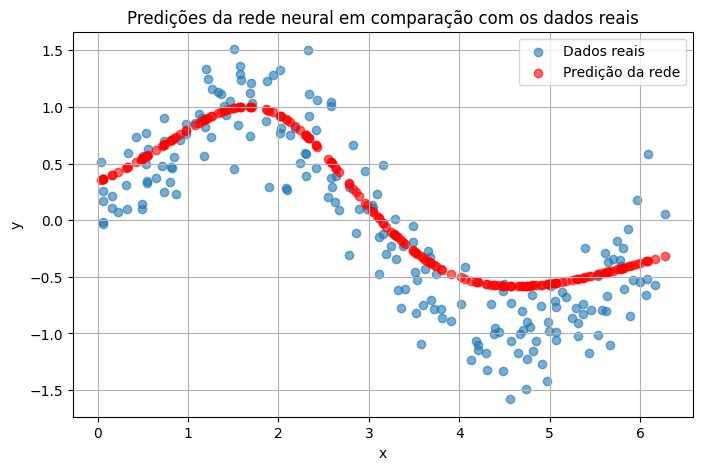
\includegraphics[width=\textwidth]{./0803_imgs/png-241110-154527304-12037654268696582542.png}
	%\legend{Fonte: Gerado peloComando da atividade}
	\end{minipage}
	\hfill
	\begin{minipage}{0.45\textwidth}
	\centering
	\caption{Treinando com 5k épocas.}\label{tarefa02:5000:predicoes}
	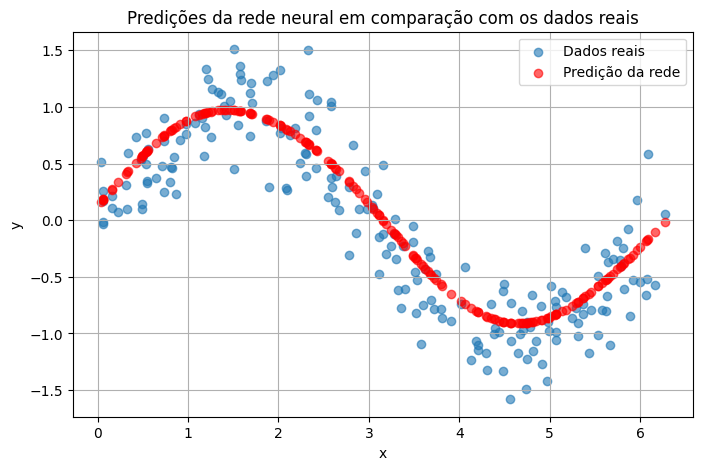
\includegraphics[width=\textwidth]{./0803_imgs/png-241110-154628196-17784737572676737911.png}
	%\legend{Fonte: \citeonline[p. 24]{araujo2012}}
	\end{minipage}
    \vspace{1Ex}
    \begin{minipage}{0.45\textwidth}
        \centering
        \caption{Treinando com 10k épocas.}\label{tarefa02:10000:predicoes}
        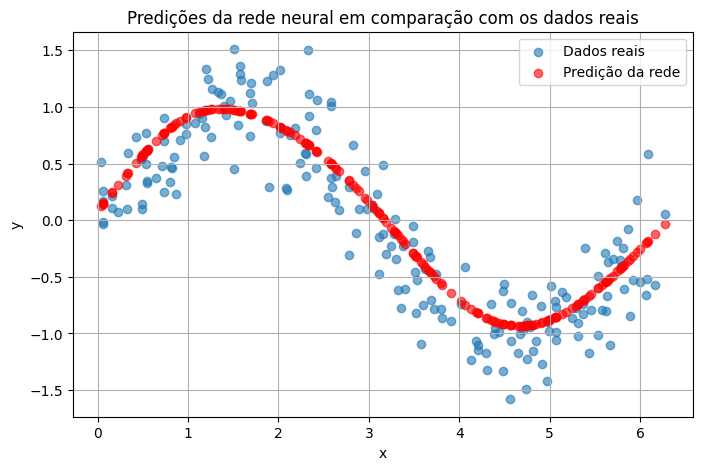
\includegraphics[width=\textwidth]{./0803_imgs/png-241110-154812342-18762265025268743.png}
        %\legend{Fonte: \citeonline[p. 24]{araujo2012}}
    \end{minipage}
	\hfill
	\begin{minipage}{0.45\textwidth}
	\centering
	\caption{Treinando com 20k épocas.}\label{tarefa02:20000:predicoes}
	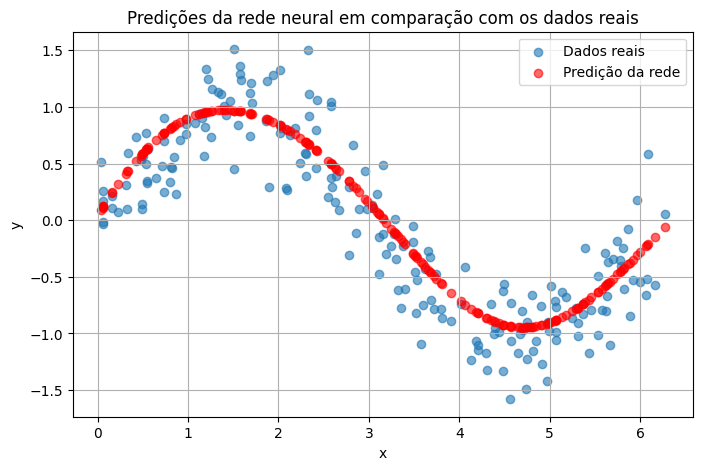
\includegraphics[width=\textwidth]{./0803_imgs/png-241110-155300412-9439382542521307108.png}
	%\legend{Fonte: \citeonline[p. 24]{araujo2012}}
	\end{minipage}
\end{figure}

\begin{figure}
	\centering
	\caption{Curvas de perdas durante o treinamento para as diferentes 
	redes}\label{tarefa02:figura:curvas}
	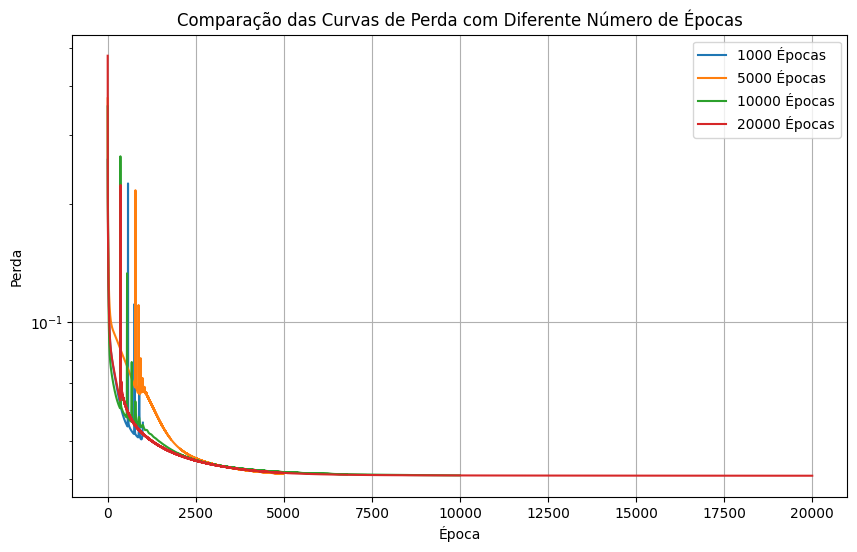
\includegraphics[width=0.7\linewidth]{./0803_imgs/png-241110-160937603-16503693892993531452.png}
\end{figure}

\begin{table}[htb]
	\caption{Perda de teste para as diferentes redes neurais}
	\centering
	\label{tarefa02:tabela:perdas}
\begin{tabular}{c | c}
	Rede Neural & Perda com dados de teste \\
	1k épocas  &  0.06468 \\
	5k épocas  &  0.04504 \\
	10k épocas &  0.04528 \\
	20k épocas &  0.04492
\end{tabular}
\end{table}

Após 5000 épocas de treinamento, foi observado que as redes neurais apresentam 
erros muito próximos uns dos outros. Isso indica que, a partir desse ponto, 
aumentar ainda mais o número de épocas de treinamento não traz melhorias 
significativas na capacidade preditiva das redes. Este achado é importante, 
pois sugere que as redes alcançaram um nível de desempenho máximo e que o 
treinamento adicional pode não ser benéfico.

Um caso especial que chama a atenção é a rede neural treinada com apenas 1000 
épocas. Esta rede exibe um erro de previsão significativamente maior do que as 
outras redes, indicando um caso de "underfitting". Underfitting ocorre quando 
um modelo é muito simples para capturar os padrões complexos nos dados, 
resultando em um desempenho de previsão inferior.

Uma observação secundária interessante é a comparação entre a rede treinada com 
a função de ativação Gelu por 1000 épocas e a rede treinada com a função de 
ativação sigmóide. Parece que ambas as redes têm capacidades preditivas 
semelhantes, apesar da diferença na função de ativação e no número de épocas de 
treinamento. Isso pode sugerir que, neste caso específico, a função de ativação 
Gelu com menos épocas de treinamento pode alcançar um desempenho comparável ao 
sigmóide.

Em resumo, esta análise destaca a importância de monitorar o desempenho das 
redes neurais em diferentes pontos do treinamento. Mostra que o underfitting 
pode ocorrer com menos épocas de treinamento e que diferentes funções de 
ativação podem ter impactos variados no desempenho do modelo. Os resultados 
também sugerem que, após um certo número de épocas, a melhoria no desempenho da 
rede neural pode ser marginal, indicando que a otimização adicional pode não 
ser necessária.
